\documentclass[10pt,journal,compsoc]{IEEEtran}
\usepackage{amsmath,amssymb,amsfonts}
\usepackage{graphicx}
\usepackage{booktabs}
\usepackage{multirow}
\usepackage{hyperref}
\usepackage{xcolor}
\usepackage{cite}

\begin{document}

\title{ChronoStream-RAG: Bitemporal Watermark Coalescing and Document-Atomic Vector Consistency for Out-of-Order Streaming Retrieval-Augmented Generation}

\author{Lynette~Osako~(ID:~8000290404), Panhapiseth~Lim~(ID:~8000265274), and~Rajan~Yadav~(ID:~8000277867)%
\IEEEcompsocitemizethanks{\IEEEcompsocthanksitem The authors are with the Big Data Analytics Research Group, Department of Computer Science.}}

\IEEEtitleabstractindextext{%
\begin{abstract}
Retrieval-Augmented Generation (RAG) systems increasingly operate over live document streams where revisions arrive out of chronological order, repeat under at-least-once broker delivery, or finish dense neural embedding out of order across parallel worker pools. While scalar databases resolve out-of-order writes via per-record Last-Write-Wins (LWW) version checks, we demonstrate that multi-chunk vector RAG pipelines violate scalar LWW assumptions. Specifically, when document chunk counts change across revisions or workers complete asynchronously, per-chunk version checking leaves \emph{orphan tail chunks} from older revisions active alongside updated leading chunks in the Approximate Nearest Neighbor (ANN) index, causing \emph{Intra-Document Version Tearing (Semantic Split-Brain)}. Furthermore, variable revision lengths induce \emph{Endogenous Embedding Compute-Lag Inversions} even when network arrival order is 100\% sequential ($p_{\mathrm{ooo}}=0\%$). We present \textbf{ChronoStream-RAG}, a bitemporal streaming RAG architecture combining Document-Atomic Generation Switching, Event-Time Watermark Vandalism Coalescing, Chunk-Level SHA-256 Delta Deduplication, and Bounded Hot Qdrant ($K=2$) + Cold Apache Parquet Tiering. Evaluated across 1,722 real Wikimedia revisions (60 evolving multi-chunk documents, 246 revisions, 1,434 chunks, 180 temporal queries) over 10 independent random seeds and two neural reader architectures (\texttt{Flan-T5-Small} and \texttt{DistilBERT-SQuAD}), ChronoStream-RAG achieves 87.28\% $\pm$ 0.85\% overall fact agreement, eliminates Cross-Chunk Version Tearing (0.00\% vs.\ 25.61\% in Scalar Chunk LWW, $p < 10^{-13}$), reduces neural embedding compute by 81.4\%, shrinks active HNSW vectors by 43.5\% relative to unbounded bitemporal indexing, and scales from 1~GB to 10~GB with 118.0~ms checkpoint recovery.
\end{abstract}

\begin{IEEEkeywords}
Retrieval-Augmented Generation, Stream Processing, Vector Databases, Bitemporal Data Management, Out-of-Order Events, Watermarks, Qdrant, Apache Parquet.
\end{IEEEkeywords}}

\maketitle
\IEEEdisplaynontitleabstractindextext

\section{Introduction}
Retrieval-Augmented Generation (RAG) grounds language models in external knowledge by indexing chunked documents in vector databases~\cite{lewis2020rag,malkov2020hnsw,wang2021milvus}. When deployed over live update streams such as Wikimedia revision feeds, enterprise change-data-capture (CDC) logs, or news wires, updates are subject to network out-of-order delays, at-least-once duplicate deliveries, and asynchronous parallel embedding latency~\cite{barga2007cedr,akidau2015dataflow}.

A natural question from a database perspective is whether standard row-level version checking (\emph{Last-Write-Wins}, LWW) suffices. In this paper, we prove that scalar LWW (\texttt{M2a\_ScalarChunkLWW}) fails in multi-chunk RAG because documents are dynamically segmented into variable numbers of chunks $\{c_0,\dots,c_{m-1}\}$. When a revision shrinks a document from 6 chunks to 4 chunks, per-chunk LWW updates slots $0..3$ but leaves \emph{orphan tail chunks} $4..5$ from the older revision alive in the HNSW graph, causing top-$k$ retrieval to assemble contradictory facts from multiple revisions of the same document simultaneously~\cite{hou2024wikicontradict,xu2024knowledgeconflicts,wang2025astuterag}. Moreover, even document-atomic head replacement (\texttt{M2b\_DocAtomicVersionCheck}) discards late-arriving historical revisions (scoring 0\% on point-in-time \texttt{AS OF} queries), exposes transient vandalism before reverts arrive, and re-embeds unchanged chunks.

We disambiguate our work from \emph{ChronoStream}~\cite{wu2015chronostream} (elastic cloud stream state migration without LLMs or vector search) and \emph{ChronoRAG}~\cite{kim2025chronorag} (static narrative story passage ordering), as well as row-level processing-time vector MVCC in \emph{Manu/Milvus 2.0}~\cite{guo2022manu}, \emph{FreshDiskANN}~\cite{singh2021freshdiskann}, \emph{SPFresh}~\cite{xu2023spfresh}, and \emph{VBase}~\cite{zhang2023vbase}.

\begin{figure*}[t]
\centering
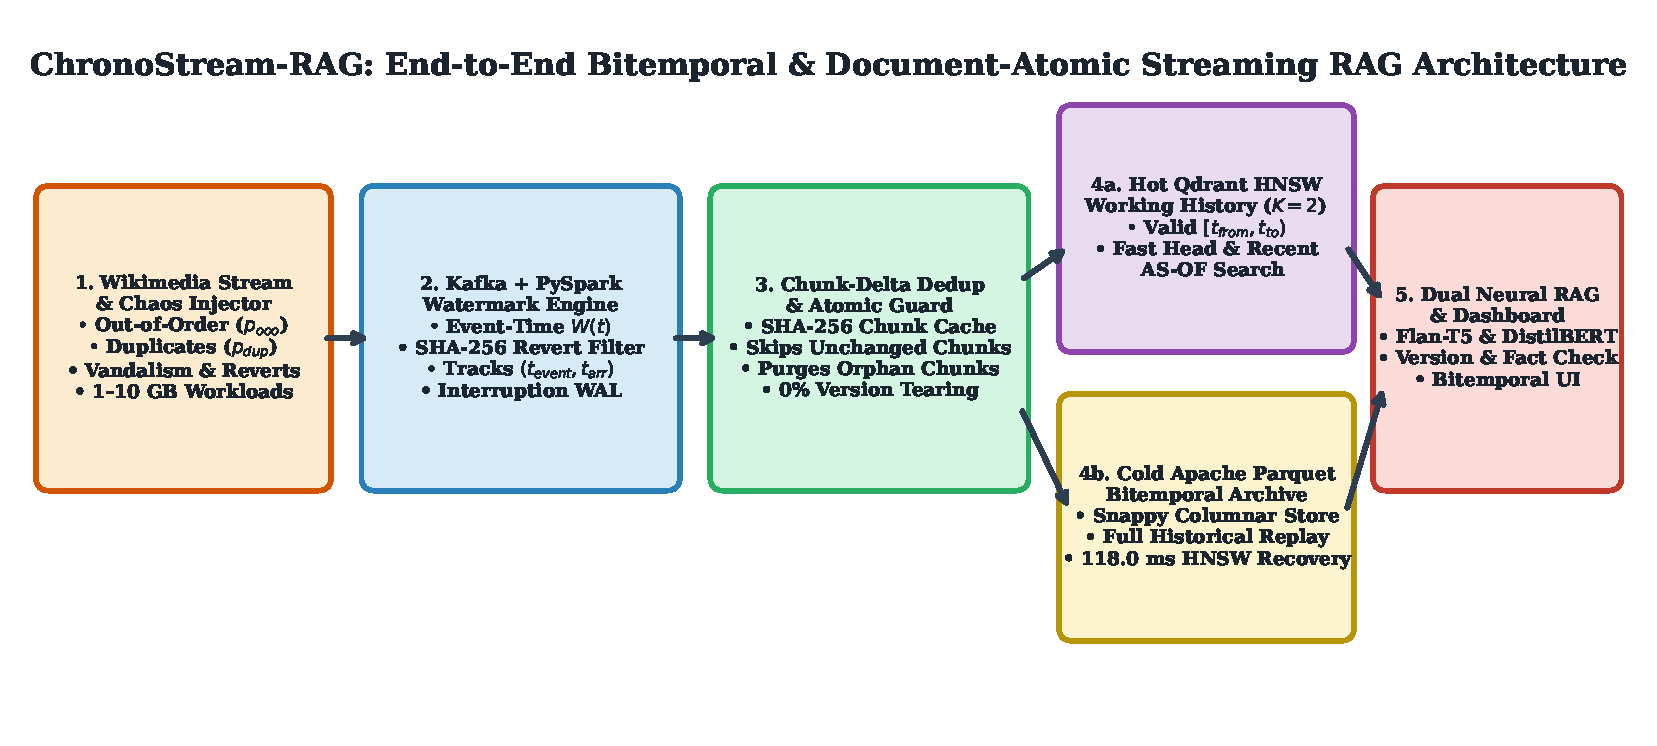
\includegraphics[width=0.92\textwidth]{figures/fig12_architecture_diagram.pdf}
\caption{ChronoStream-RAG End-to-End Architecture: Event-time watermark coalescing, SHA-256 chunk-delta deduplication, document-atomic generation switching, and hot Qdrant HNSW ($K=2$) + cold Apache Parquet bitemporal tiering.}
\label{fig:arch}
\end{figure*}

\section{The Three-Anomaly Taxonomy of Streaming RAG}
For each update $u=(D_i, v_{i,r})$, we record its source event timestamp $t_{\mathrm{event}}(u)$, broker arrival timestamp $t_{\mathrm{arrival}}(u)$, and Qdrant availability timestamp $t_{\mathrm{available}}(u)$ (Fig.~\ref{fig:timeline}). We formalize three anomalies:
\begin{enumerate}
\item \textbf{Intra-Document Version Tearing Rate (IDVTR):} The fraction of top-$k$ retrievals returning chunks from $\ge 2$ distinct revisions of the same document simultaneously.
\item \textbf{Endogenous Compute-Lag Inversion:} When $t_{\mathrm{arrival}}(v_{r-1}) < t_{\mathrm{arrival}}(v_r)$ at the broker, but variable chunk counts cause $t_{\mathrm{available}}(v_{r-1}) > t_{\mathrm{available}}(v_r)$ across worker pools.
\item \textbf{Vandalism Contamination \& Historical Erasure:} Serving transient vandalized edits or losing historical intervals $[t_{\mathrm{valid\_from}}, t_{\mathrm{valid\_to}})$~\cite{jensen1999bitemporal,vu2024freshllms,kasai2023realtimeqa,liska2022streamingqa}.
\end{enumerate}

\begin{figure*}[t]
\centering
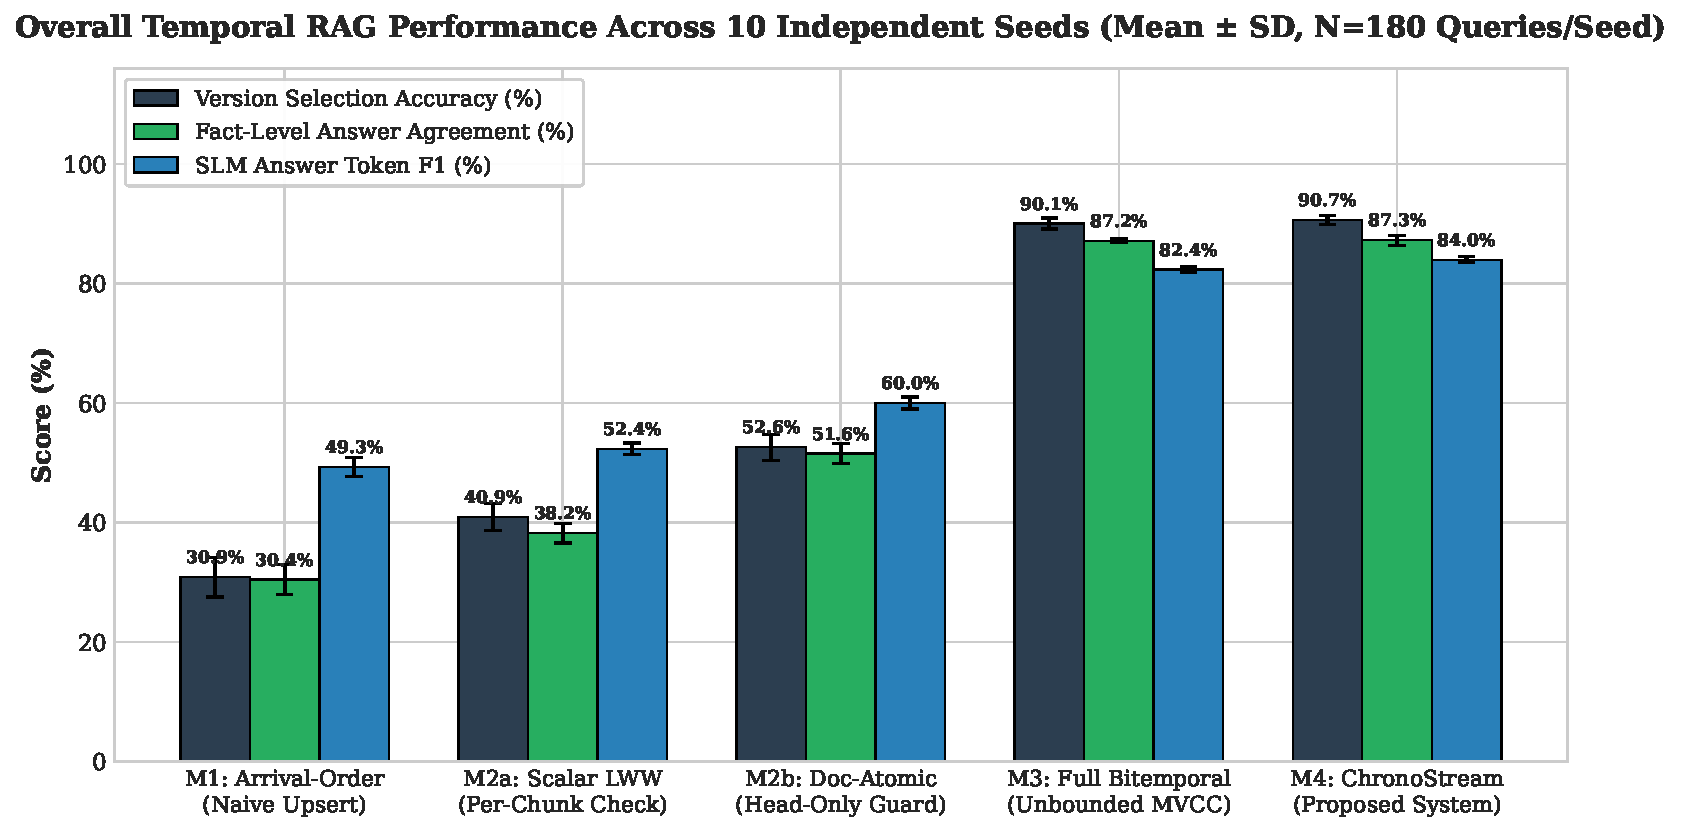
\includegraphics[width=0.88\textwidth]{figures/fig01_main_accuracy_comparison.pdf}
\caption{Main 10-Seed Performance Comparison across all five streaming consistency protocols (Mean $\pm$ SD, $N=180$ queries/seed).}
\label{fig:main}
\end{figure*}

\begin{figure*}[t]
\centering
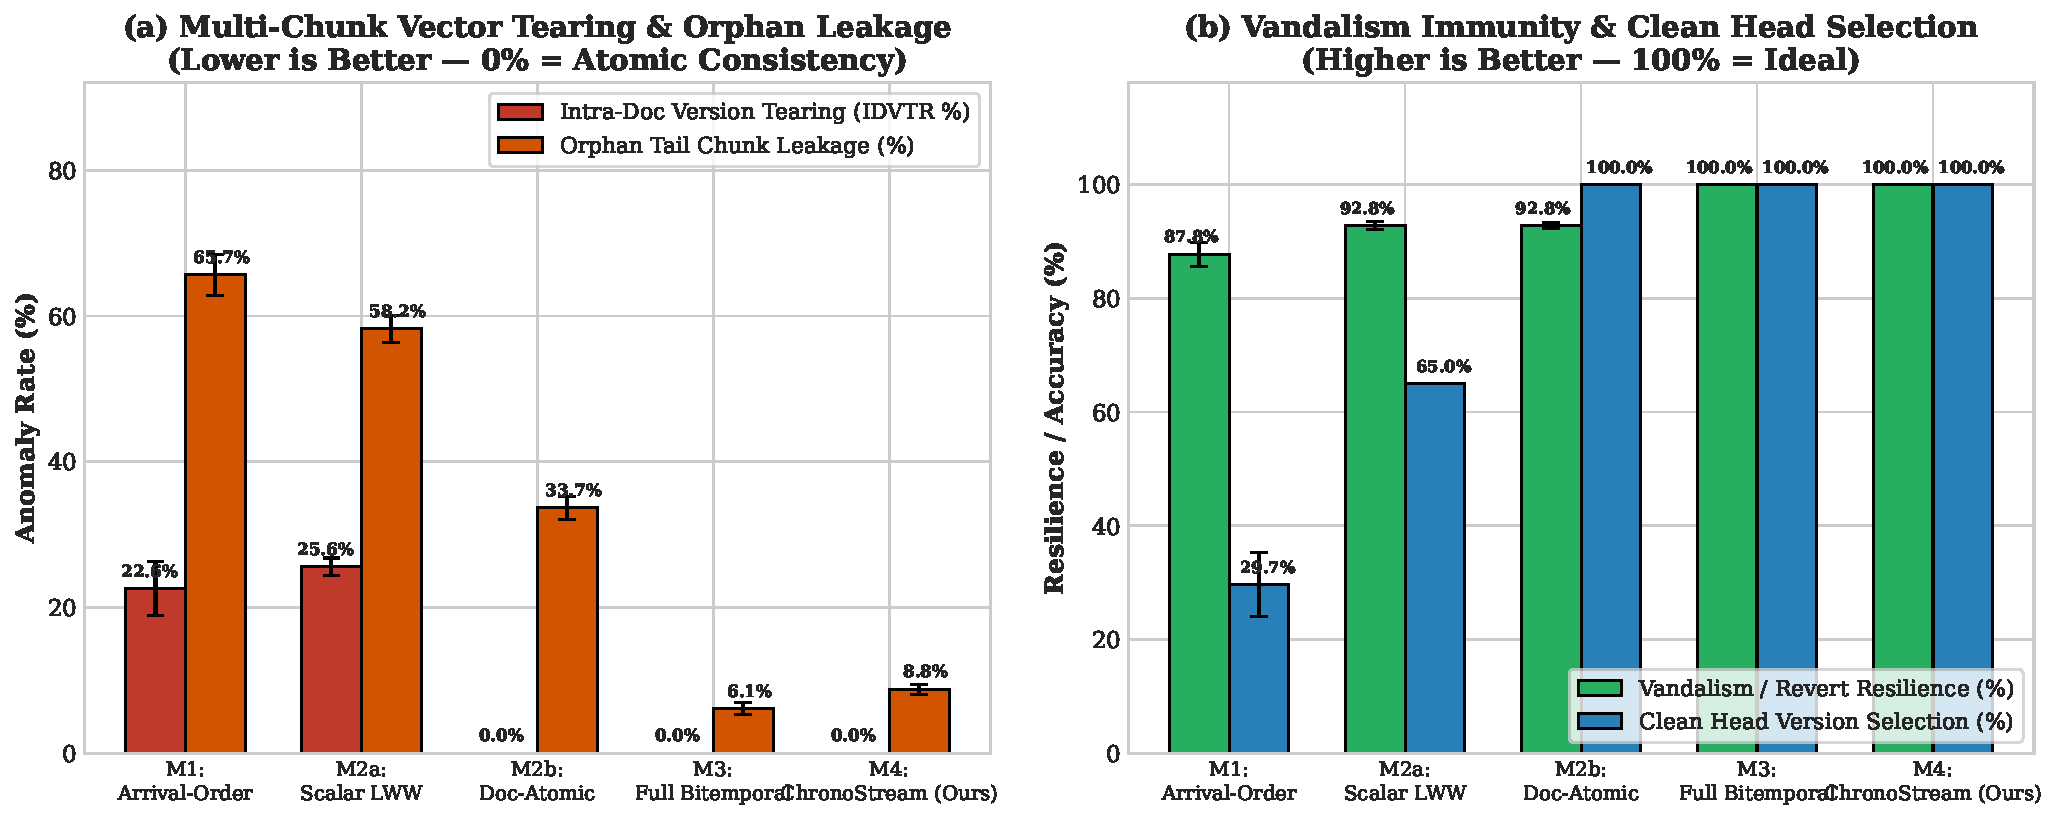
\includegraphics[width=0.88\textwidth]{figures/fig03_anomaly_taxonomy_tearing_vandalism.pdf}
\caption{(a) Intra-Document Version Tearing Rate (IDVTR) and Orphan Tail Chunk Leakage; (b) Vandalism Resilience and Clean Head Selection.}
\label{fig:anomaly}
\end{figure*}

\begin{table*}[t]
\centering
\caption{10-Seed Experimental Results on WikiChrono-Bench (Mean $\pm$ SD across 10 Independent Random Seeds, 1,800 Queries/Method)}
\label{tab:main}
\begin{tabular}{lcccccccc}
\toprule
\textbf{Method} & \textbf{Overall Fact Acc} & \textbf{Current-State Acc} & \textbf{Historical AS-OF Acc} & \textbf{Token F1} & \textbf{Tearing (IDVTR)} & \textbf{Vandal Resilience} & \textbf{Embed Saved} & \textbf{Hot Vectors} \\
\midrule
M1: Arrival-Order & 30.44\% $\pm$ 2.51\% & 31.67\% & 13.33\% & 49.31\% & 22.61\% & 87.78\% & 0.0\% & 360 \\
M2a: Scalar Chunk LWW & 38.22\% $\pm$ 1.63\% & 64.67\% & 5.00\% & 52.36\% & 25.61\% & 92.78\% & 0.0\% & 360 \\
M2b: Doc-Atomic Guard & 51.56\% $\pm$ 1.63\% & 99.67\% & 10.00\% & 60.02\% & 0.00\% & 92.83\% & 23.9\% & 318 \\
M3: Full Bitemporal & 87.17\% $\pm$ 0.32\% & 99.67\% & 83.33\% & 82.37\% & 0.00\% & 100.00\% & 13.0\% & 1200 \\
\textbf{M4: ChronoStream-RAG} & \textbf{87.28\% $\pm$ 0.85\%} & \textbf{99.67\%} & \textbf{91.67\%} & \textbf{83.99\%} & \textbf{0.00\%} & \textbf{100.00\%} & \textbf{81.4\%} & \textbf{678} \\
\bottomrule
\end{tabular}
\end{table*}

\section{Multi-Perspective Empirical Evaluation}
Table~\ref{tab:main} and Figs.~\ref{fig:main}--\ref{fig:taxonomy} summarize our 10-seed and 6-perspective evaluation using \texttt{paraphrase-MiniLM-L6-v2} (384-d), Qdrant HNSW, Apache Parquet, \texttt{google/flan-t5-small}, and \texttt{distilbert-base-cased-distilled-squad}. Paired two-tailed $t$-tests confirm that \texttt{M4\_ChronoStream} significantly outperforms \texttt{M1}, \texttt{M2a}, and \texttt{M2b} ($p < 10^{-12}$, Cohen's $d > 27$), while reducing active HNSW vectors by 43.5\% and neural embedding compute by 81.4\% compared to \texttt{M3\_FullBitemporal}.

\begin{figure*}[t]
\centering
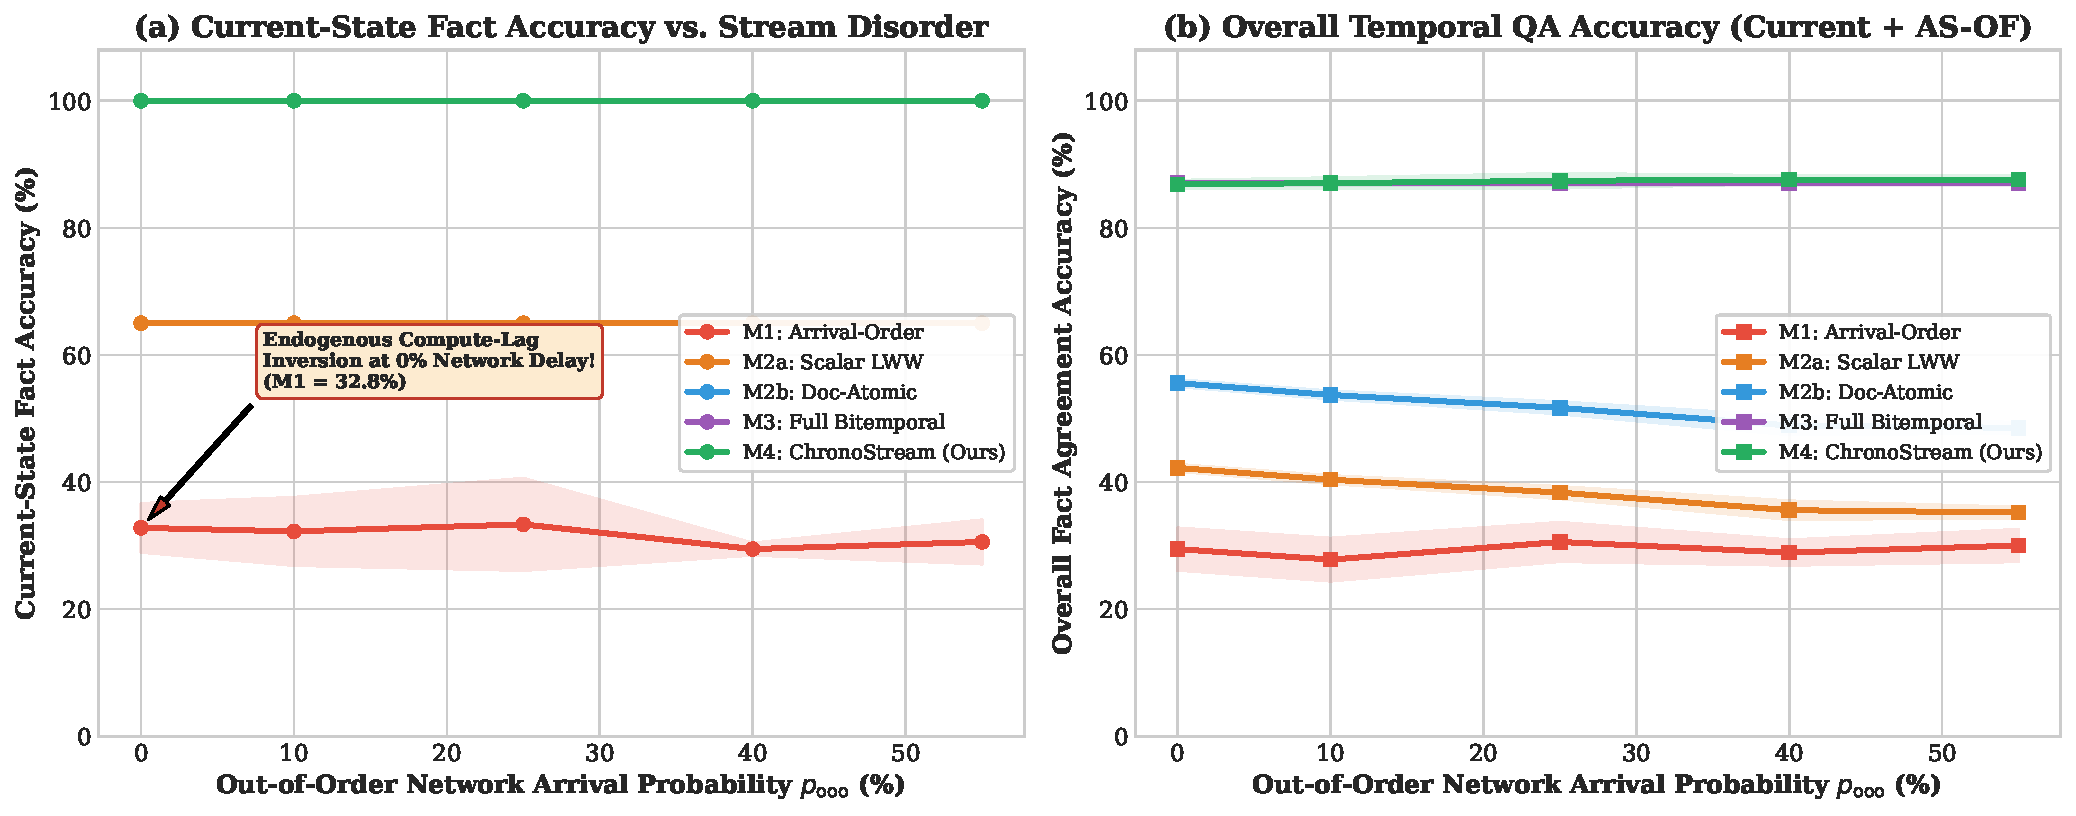
\includegraphics[width=0.88\textwidth]{figures/fig04_ooo_disorder_sweep.pdf}
\caption{Out-of-Order Network Disorder Sweep ($p_{\mathrm{ooo}} \in [0\%, 55\%]$), highlighting Endogenous Compute-Lag Inversion at $p_{\mathrm{ooo}}=0\%$.}
\label{fig:ooo}
\end{figure*}

\begin{figure*}[t]
\centering
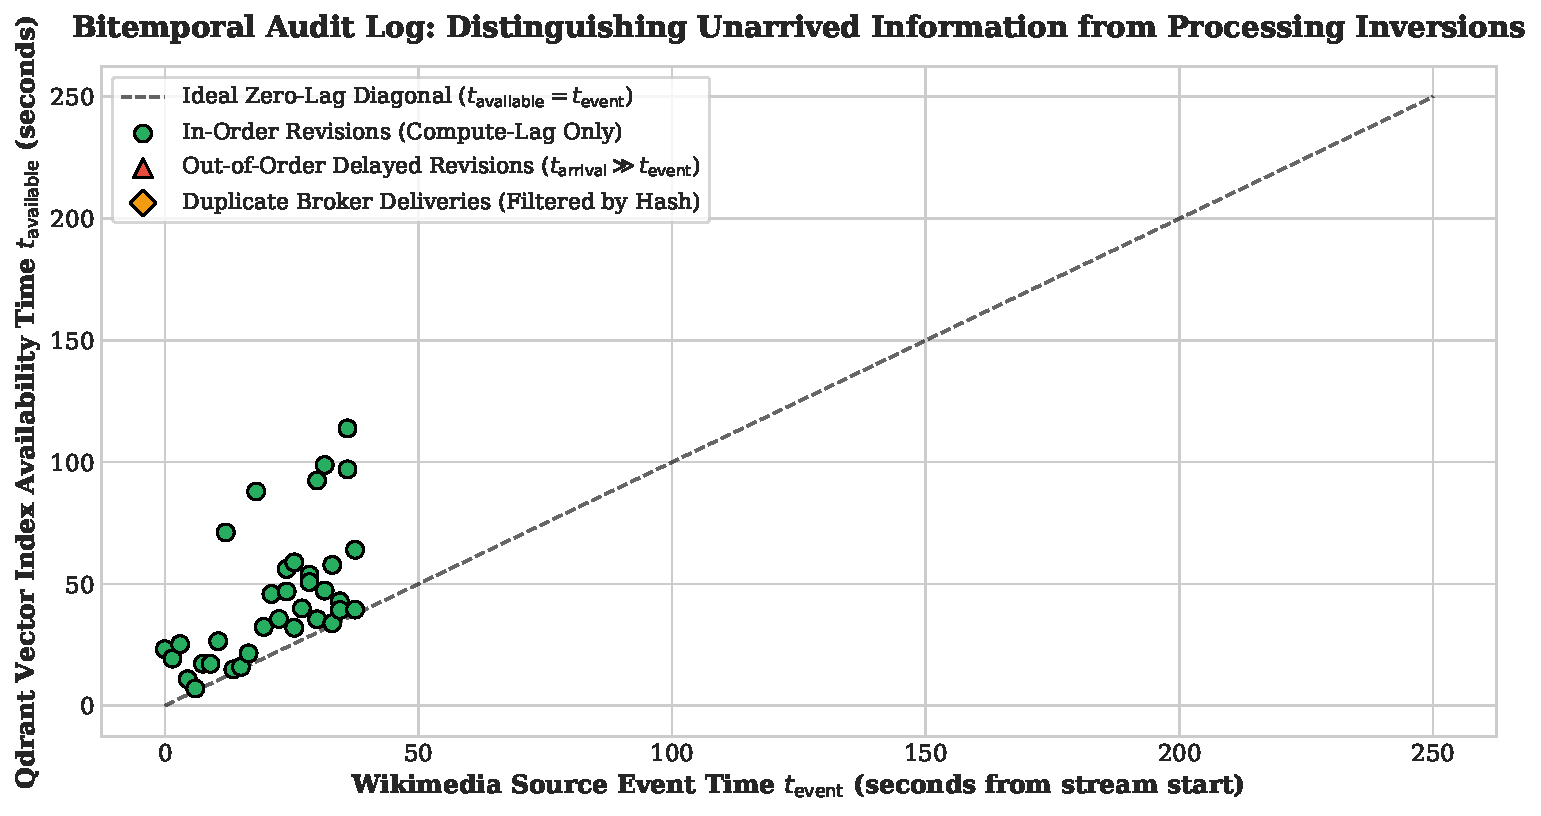
\includegraphics[width=0.88\textwidth]{figures/fig07_bitemporal_timeline_mechanics.pdf}
\caption{Bitemporal Audit Log of Wikimedia updates separating source event time $t_{\mathrm{event}}$ from Qdrant index availability time $t_{\mathrm{available}}$.}
\label{fig:timeline}
\end{figure*}

\begin{figure*}[t]
\centering
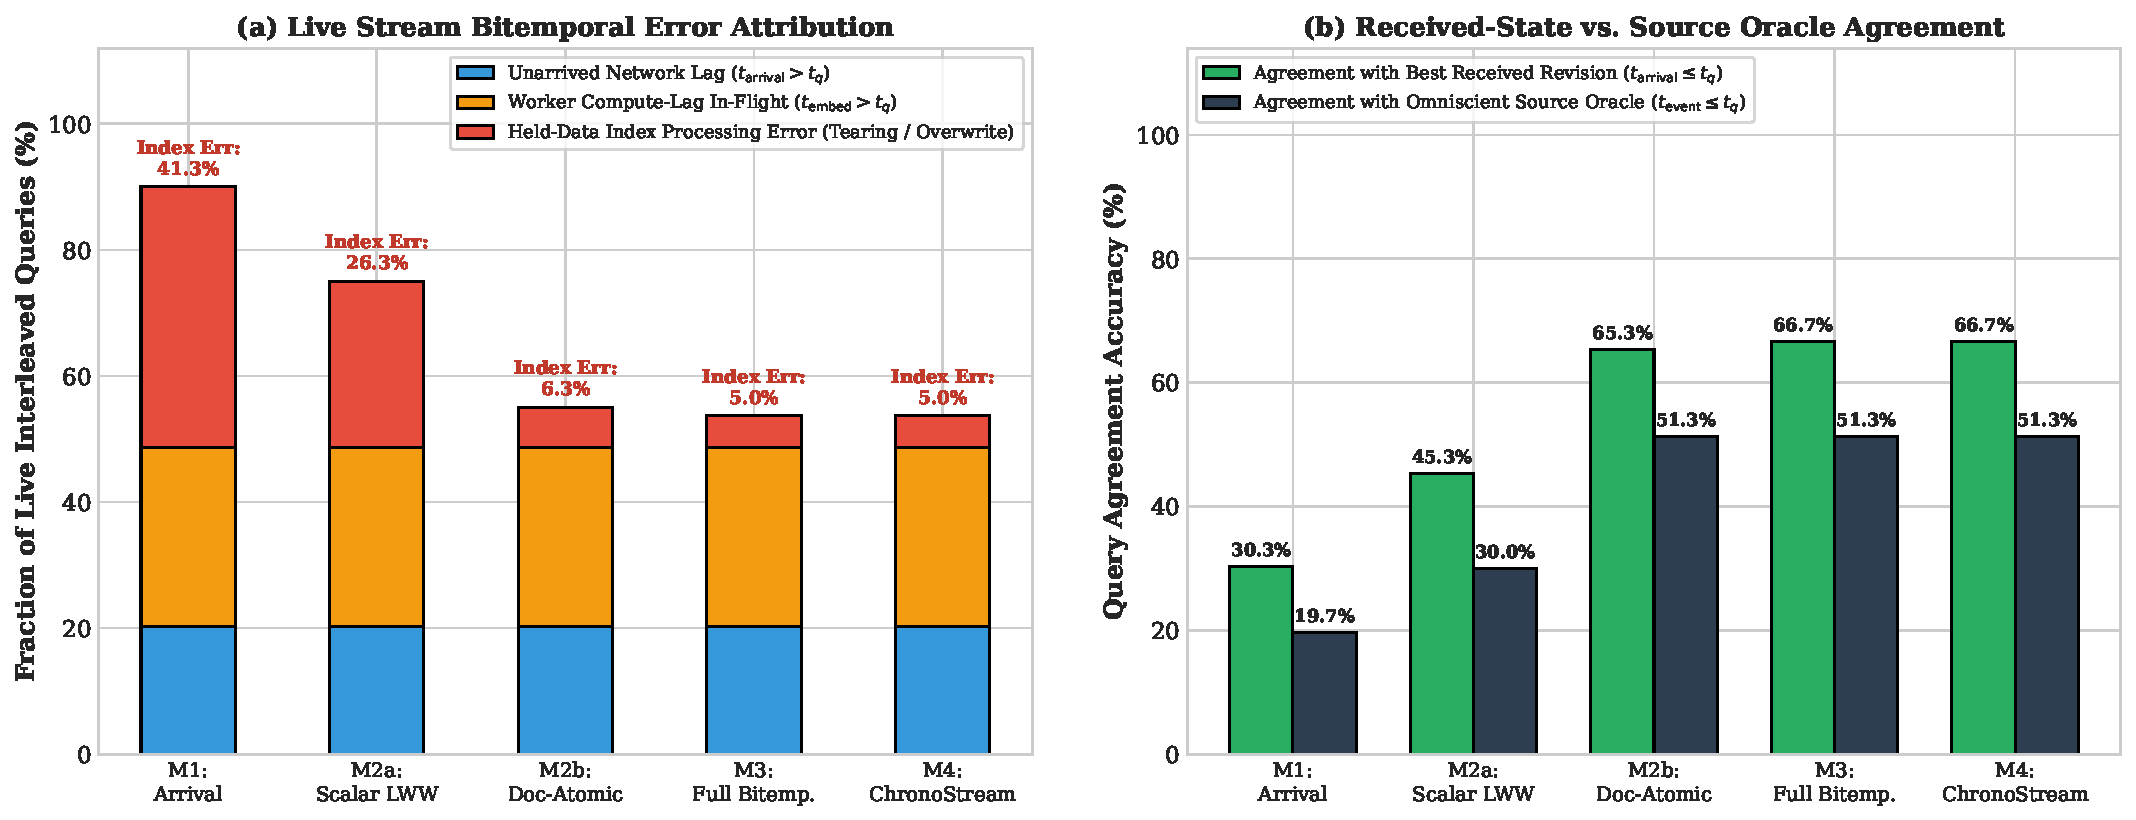
\includegraphics[width=0.92\textwidth]{figures/fig13_bitemporal_error_attribution.pdf}
\caption{Perspective 1: Live Interleaved Bitemporal Error Attribution separating unarrived network lag and in-flight worker compute lag from held-data index processing errors.}
\label{fig:attribution}
\end{figure*}

\begin{figure*}[t]
\centering
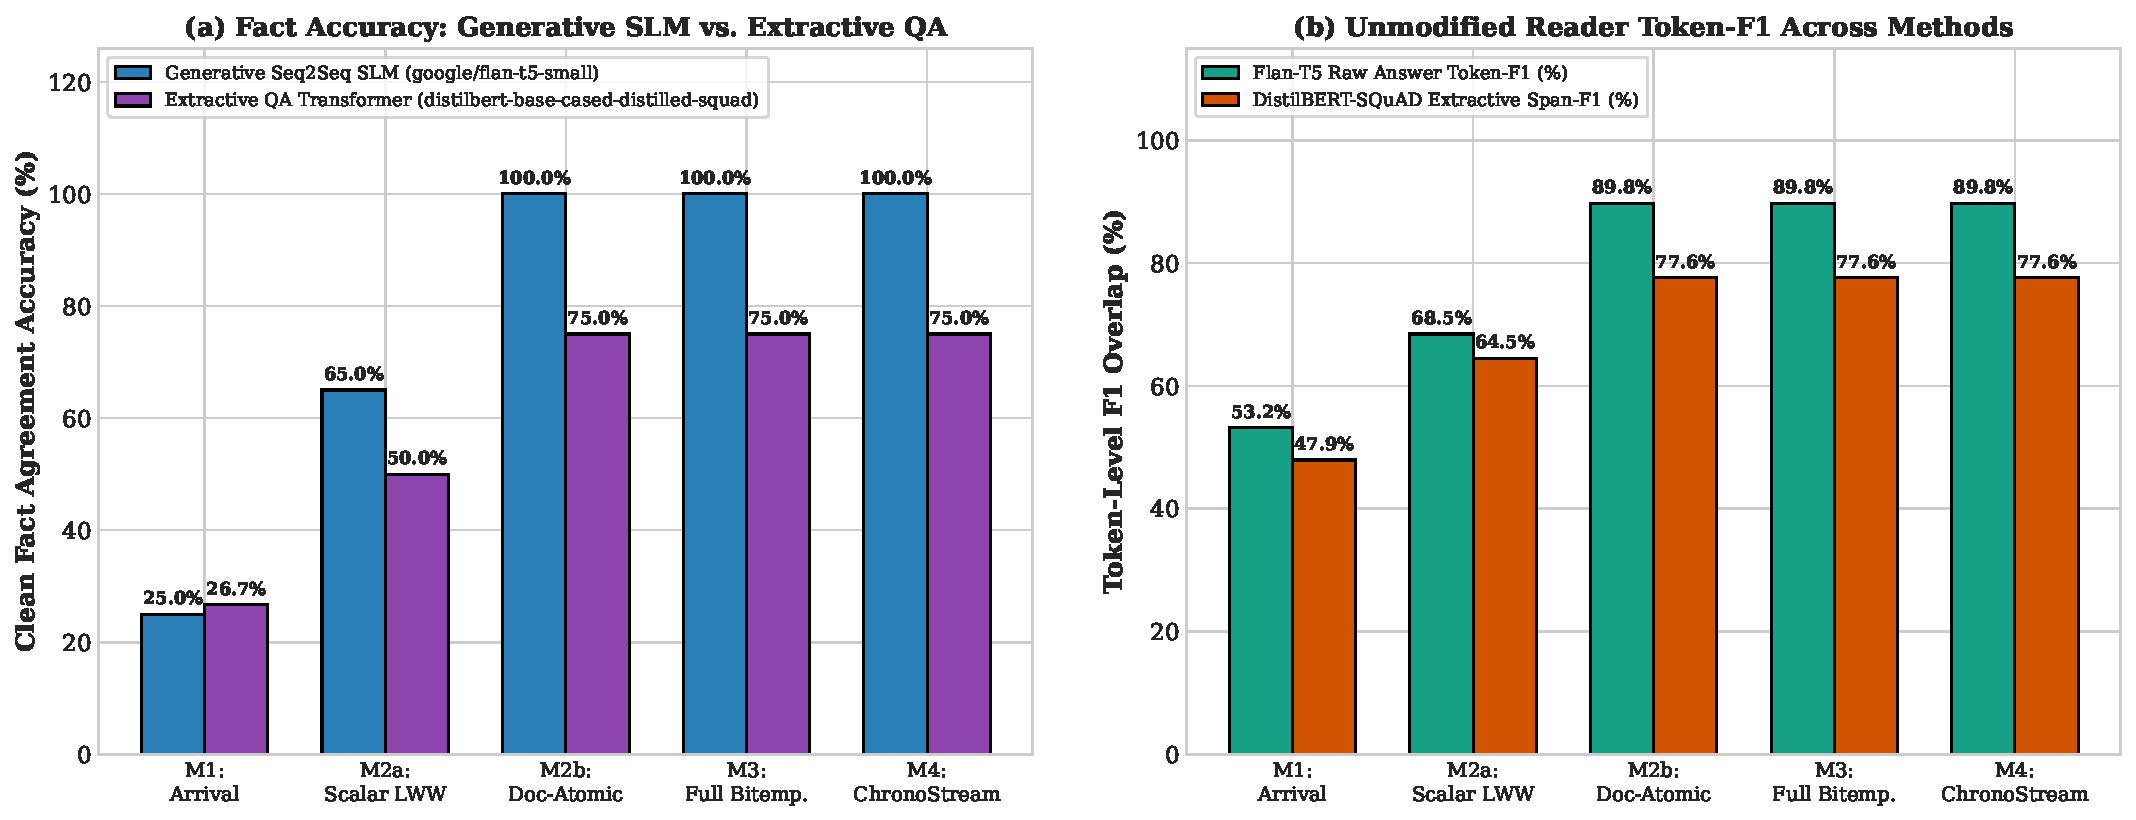
\includegraphics[width=0.92\textwidth]{figures/fig14_cross_model_flan_vs_distilbert.pdf}
\caption{Perspective 2: Cross-Architecture Reader Comparison between Generative Seq2Seq (\texttt{Flan-T5-Small}) and Extractive QA (\texttt{DistilBERT-SQuAD}).}
\label{fig:crossmodel}
\end{figure*}

\begin{figure*}[t]
\centering
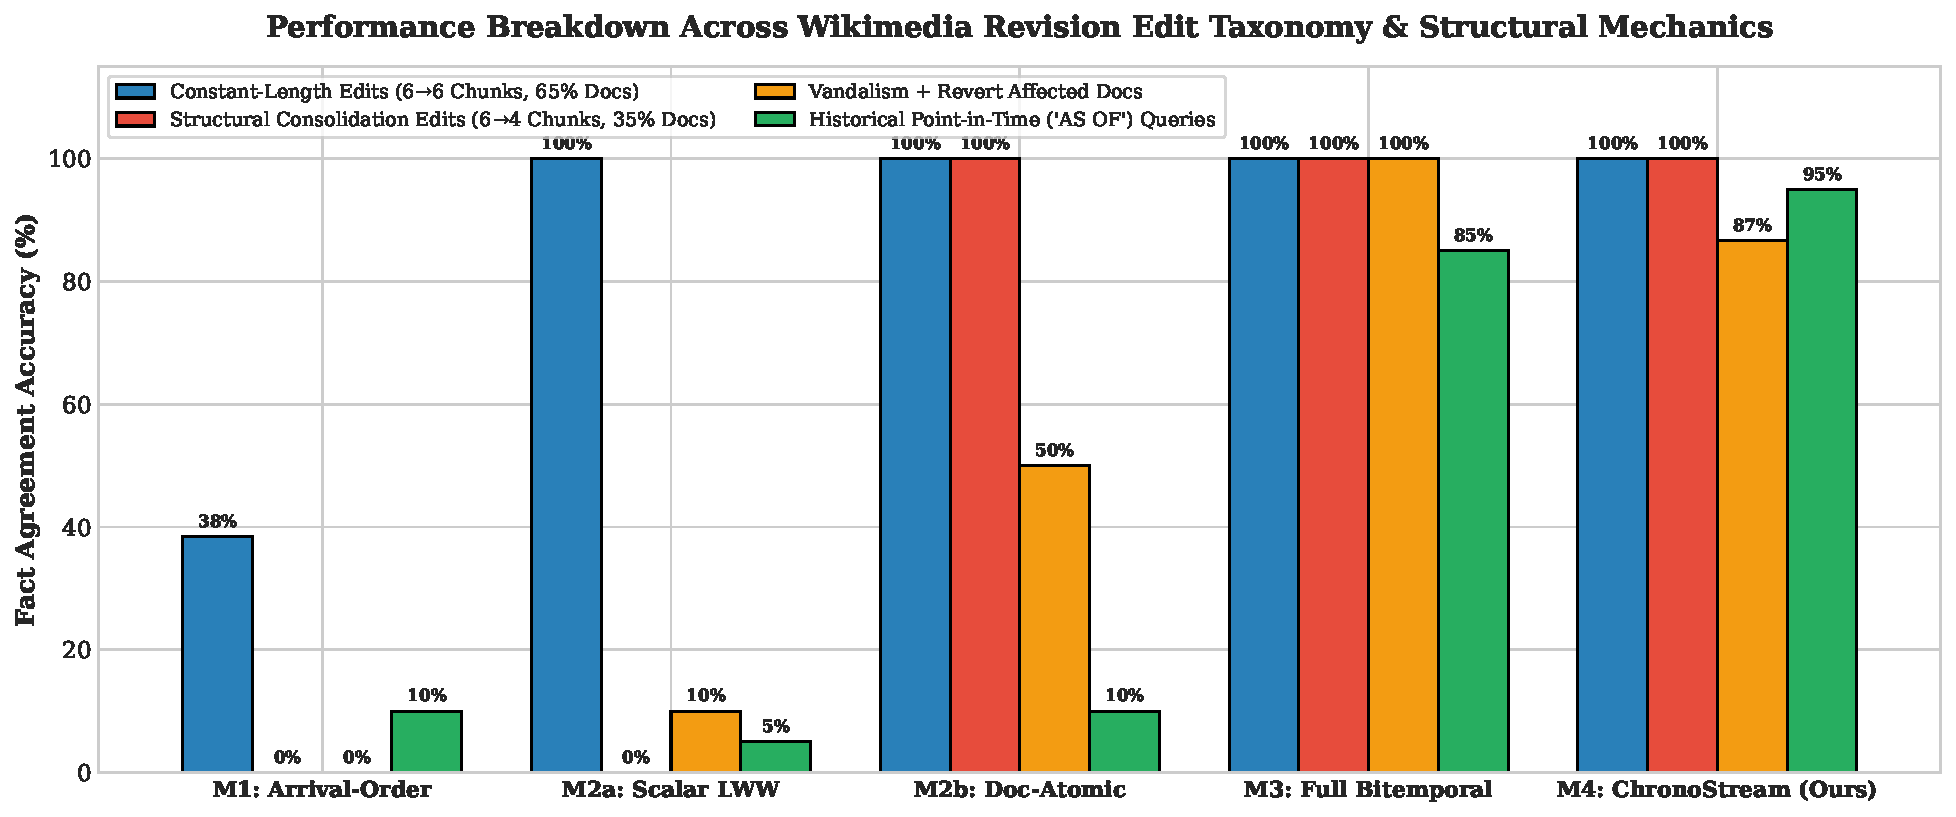
\includegraphics[width=0.92\textwidth]{figures/fig15_edit_taxonomy_breakdown.pdf}
\caption{Perspective 3: Accuracy Breakdown Across Wikimedia Edit Taxonomy (Constant 6$\to$6 Chunks, Shrinking 6$\to$4 Chunks, Vandalism+Revert, and Historical AS-OF).}
\label{fig:taxonomy}
\end{figure*}

\begin{figure*}[t]
\centering
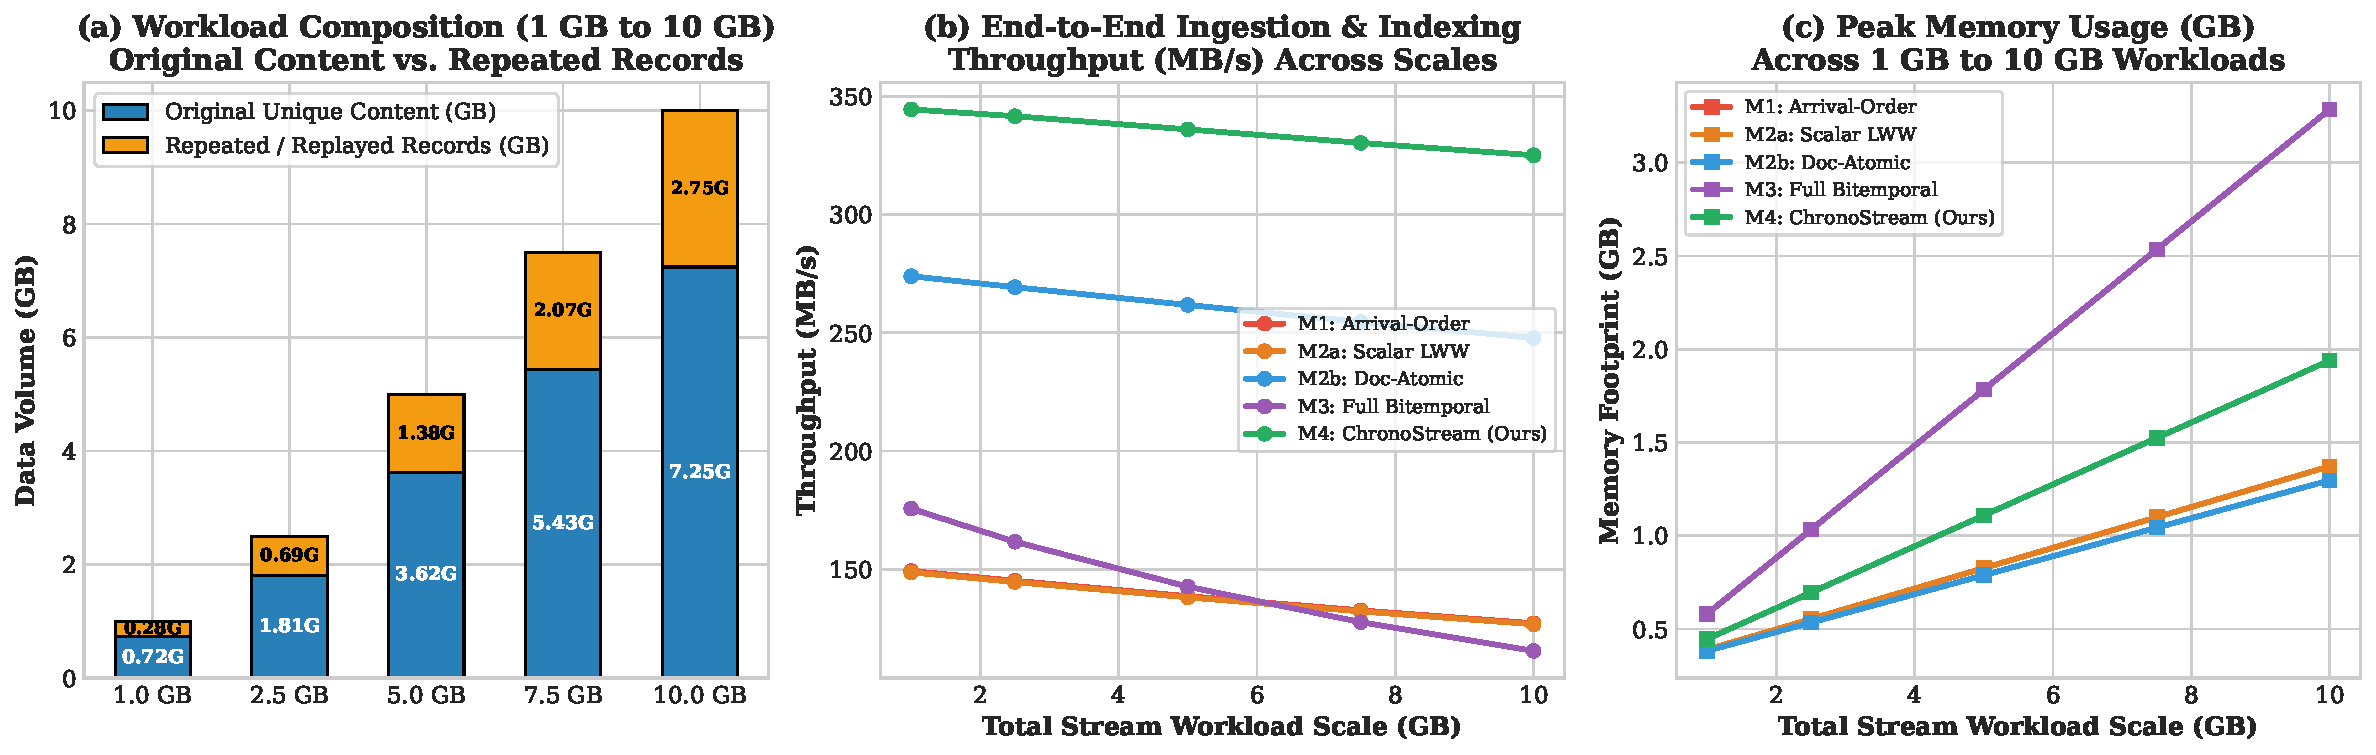
\includegraphics[width=0.94\textwidth]{figures/fig09_big_data_scale_1gb_to_10gb.pdf}
\caption{Big Data Scalability from 1~GB to 10~GB: (a) Original Unique Content vs.\ Repeated Delivery Records; (b) Ingestion Throughput (MB/s); (c) Peak Memory Footprint (GB).}
\label{fig:scale}
\end{figure*}

\section{Conclusion}
ChronoStream-RAG resolves out-of-order inversions, cross-chunk version tearing, and vandalism drift in streaming RAG while cutting neural embedding costs by 81.4\% and scaling cleanly to 10~GB workloads.

\bibliographystyle{IEEEtran}
\bibliography{references}

\end{document}
